%!TEX root = ../../book_ML.tex
\addtocontents{toc}{\protect\newpage}
\chapter{Hồi quy logistic}
\label{cha:logisticregression}
\section{Giới thiệu}

\index{hồi quy logistic -- logistic regression}
\index{logistic regression -- hồi quy logistic}
\subsection{Nhắc lại hai mô hình tuyến tính}
Hai mô hình tuyến tính đã thảo luận trong cuốn sách này, hồi quy tuyến tính và
PLA, đều có thể viết chung dưới dạng $y = f(\bx^T\bw)$ trong đó $f(s)$ là một
hàm kích hoạt. Trong hồi quy tuyến tính $f(s) = s$, tích vô hướng $\bx^T\bw$
được trực tiếp sử dụng để dự đoán đầu ra $y$. Mô hình này phù hợp nếu ta cần dự
đoán một đầu ra không bị chặn. PLA có đầu ra chỉ nhận một trong hai giá trị $1$
hoặc $-1$ với hàm kích hoạt $f(s) = \sgn(s)$ phù hợp với các bài toán phân loại
nhị phân. Trong chương này, chúng ta sẽ thảo luận một mô hình tuyến tính với một
hàm kích hoạt khác, thường được áp dụng cho các bài toán phân loại nhị phân.
Trong mô hình này, đầu ra có thể được biểu diễn dưới dạng xác suất. Ví dụ, xác
suất thi đỗ nếu biết thời gian ôn thi, xác suất ngày mai có mưa dựa trên những
thông tin đo được trong ngày hôm nay,... Mô hình này có tên là \textit{hồi quy
logistic}. Mặc dù trong tên có chứa từ \textit{hồi quy}, phương pháp này thường
được sử dụng nhiều hơn cho các bài toán phân loại.


\subsection{Một ví dụ nhỏ}
% ******************************************************************************
\begin{table}[]
\centering
\caption{Thời gian ôn thi và kết quả thi của 20 sinh viên. }
\label{tab:10_1}
\begin{tabular}{|c|c||c|c||c|c||c|c|}
\hline
\textbf{Số giờ} & \textbf{Đậu?} & \textbf{Số giờ} & \textbf{Đậu?} & \textbf{Số giờ} & \textbf{Đậu?} & \textbf{Số giờ} & \textbf{Đậu?} \\ \hline \hline
0.5            & 0             & 0.75           & 0             & 1              & 0             & 1.25           & 0             \\ \hline
1.5            & 0             & 1.75           & 0             & 1.75           & 1             & 2              & 0             \\ \hline
2.25           & 1             & 2.5            & 0             & 2.75           & 1             & 4              & 0             \\ \hline
3.25           & 1             & 3.5            & 0             & 4              & 1             & 4.25           & 1             \\ \hline
4.5            & 1             & 4.75           & 1             & 5              & 1             & 5.5            & 1             \\ \hline
\end{tabular}
\end{table}
% ******************************************************************************

Xét một ví dụ về quan hệ giữa thời gian ôn thi và kết quả của 20 sinh
viên trong Bảng~\ref{tab:10_1}. Bài toán đặt ra là từ dữ liệu này hãy
xây dựng mô hình đánh giá khả năng đỗ của một sinh viên dựa trên thời gian
ôn tập. Dữ liệu trong Bảng~\ref{tab:10_1} được mô tả trên Hình \ref{fig:10_1}.
Nhìn chung, thời gian học càng nhiều thì khả năng đỗ càng cao. Tuy nhiên, không
có một ngưỡng thời gian học nào giúp phân biệt rạch ròi việc đỗ/trượt . Nói cách
khác, dữ liệu của hai tập này là không tách biệt tuyến tính, và vì vậy PLA sẽ
không hữu ích. Tuy nhiên, thay vì dự đoán chính xác hai giá trị đỗ/trượt,
ta có thể dự đoán xác suất để một sinh viên thi đỗ dựa trên thời gian ôn thi.

\begin{figure}[t]
% caption on side
\floatbox[{\capbeside\thisfloatsetup{capbesideposition={right,top},capbesidewidth=6cm}}]{figure}[\FBwidth]
{\caption{
Ví dụ về kết quả thi dựa trên số giờ ôn tập. Trục hoành thể hiện thời gian ôn tập của mỗi sinh viên, trục tung gồm hai giá trị 0/fail (các điểm hình tròn) và 1/pass (các điểm hình vuông).
}
\label{fig:10_1}}
{ % figure here
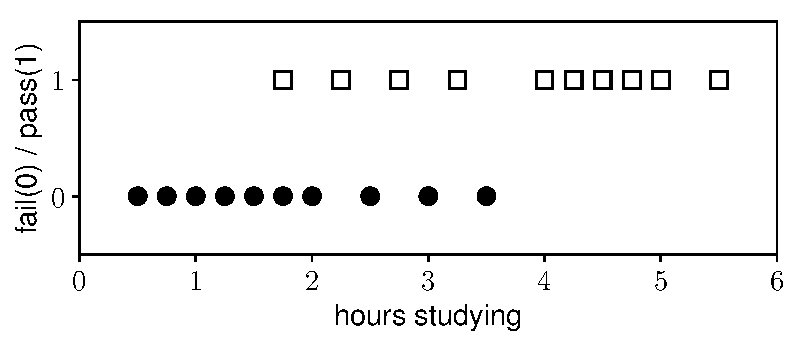
\includegraphics[width=.5\textwidth]{ebookML_src/src/logistic_regression/ex1.pdf}
}
\end{figure}


\subsection{Mô hình hồi quy logistic}
% Đầu ra dự đoán của:
% \begin{itemize}
%     \item Linear Regression:
%     \begin{equation}
%         f(\bx) = \bw^T \bx
%     \end{equation}
%     \item PLA:
%     \begin{equation}
%         f(\bx) = \text{sgn}(\bx^T\bw)
%     \end{equation}
% \end{itemize}

% Đầu ra dự đoán của hồi quy logistic thường được viết dưới dạng
% \begin{equation}
%     f(\bx) = \sigma(\bx^T\bw)
% \end{equation}
% Trong đó $\sigma$ được gọi là logistic function. Một số activation cho mô hình tuyến tính được cho trong Hình \ref{fig:10_2}

% <div class="imgcap">
% <img src ="\assets\LogisticRegression\activation.png" align = "center" width = "800">
% <div class = "thecap">Hình 2: Các activation function khác nhau.</div>
% </div>
% \begin{figure}[t]
% \centering
%     % 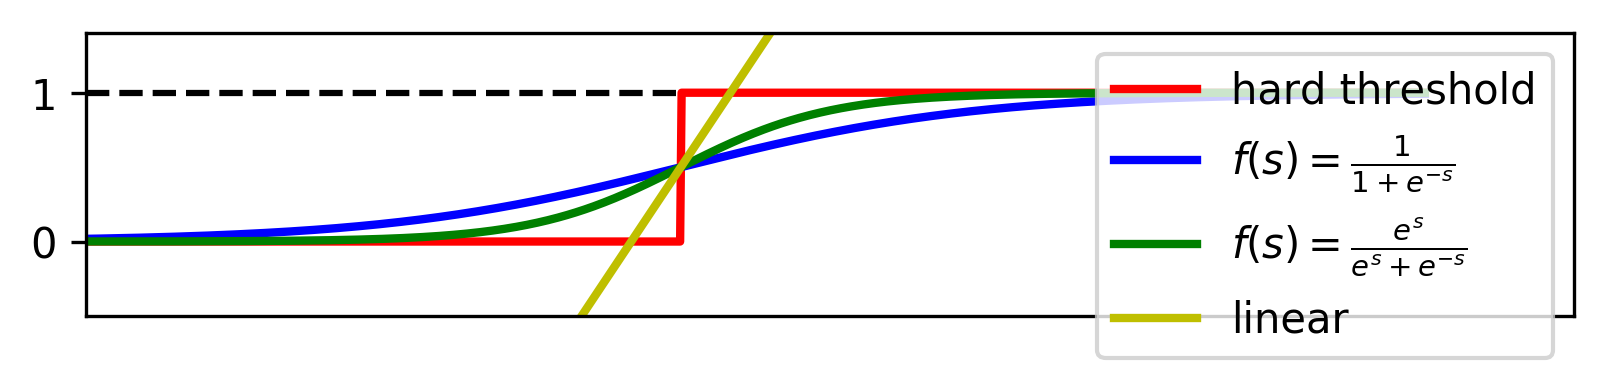
\includegraphics[width = \textwidth]{Chapters/05_NeuralNetworks/10_logisticregression/activation.png}
%     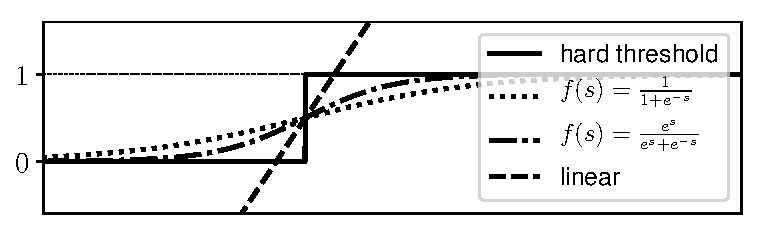
\includegraphics[width = \textwidth]{ebookML_src/src/logistic_regression/activation.pdf}
%     \caption[]{Một vài ví dụ về activation function khác nhau.}
%     \label{fig:10_2}
% \end{figure}
%% *****************************************************************************
\begin{figure}[t]
% caption on side
\floatbox[{\capbeside\thisfloatsetup{capbesideposition={right,top},capbesidewidth=5cm}}]{figure}[\FBwidth]
{\caption{
Một vài ví dụ về các hàm kích hoạt khác nhau.
}
\label{fig:10_activation}}
{ % figure here
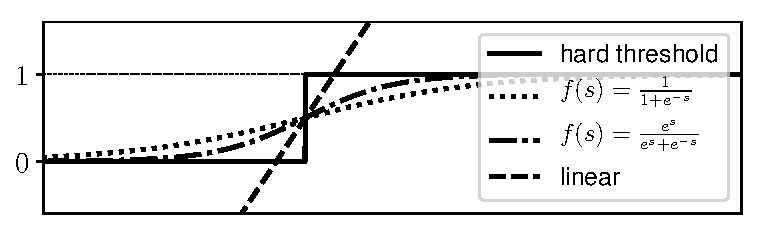
\includegraphics[width=.6\textwidth]{ebookML_src/src/logistic_regression/activation.pdf}
}
\end{figure}
%% *****************************************************************************
\index{ngưỡng -- threshold}
\index{threshold -- ngưỡng}
\index{ngưỡng cứng -- hard threshold}
\index{hard threshold -- ngưỡng cứng}
Quan sát Hình~\ref{fig:10_activation} với các hàm kích hoạt $f(s)$ khác nhau.
\begin{itemize}
\item Đường nét đứt biểu diễn một hàm kích hoạt tuyến tính không phù hợp vì
đầu ra không bị chặn. Có một cách đơn giản để đưa đầu ra về dạng bị chặn:
nếu đầu ra nhỏ hơn không thì thay bằng không, nếu đầu ra lớn hơn một thì
thay bằng một. Điểm phân chia, còn gọi là \textit{ngưỡng}, được chọn là điểm
có tung độ 0.5 trên đường thằng này. Đây cũng không phải là một lựa chọn
tốt. Giả sử có thêm một bạn {sinh viên tiêu biểu} ôn tập đến 20 giờ hoặc hơn
thi đỗ. Lúc này ngưỡng tương ứng với mốc tung độ bằng 0.5 sẽ dịch nhiều về phía
phải. Kéo theo đó, rất nhiều sinh viên thi đỗ được dự đoán là trượt. Rõ ràng
đây là một mô hình không tốt. Nhắc lại rằng hồi quy tuyến tính rất nhạy cảm
với nhiễu, ở đây là bạn {sinh viên tiêu biểu} đó.% \begin{figure}[t]
%  \centering
%      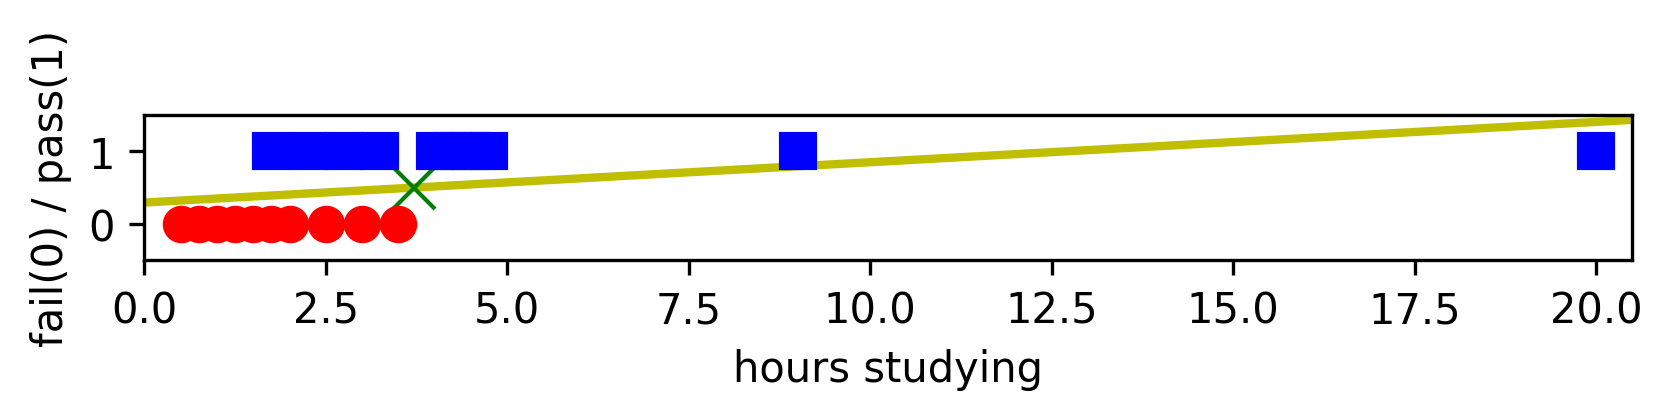
\includegraphics[width = \textwidth]{Chapters/05_NeuralNetworks/10_logisticregression/ex1_lr.png}
%      \caption[]{Tại sao Linear Regression không phù hợp?}
%      \label{fig:10_3}
%  \end{figure}

\item Đường nét liền tương tự với hàm kích hoạt của PLA\footnote{Đường này chỉ khác hàm kích hoạt của PLA ở chỗ hai nhãn là 0 và 1 thay vì -1 và 1.}. Ngưỡng dự đoán đỗ/trượt tại vị trí hàm số đổi dấu còn được gọi là \textit{ngưỡng cứng}.

% cũng thuộc dạng \textit{ngưỡng cứng} (hard threshold). PLA không hoạt động trong bài toán này vì dữ liệu đã cho không \textit{tách biệt tuyến tính}.

\item Các đường nét chấm và chấm gạch phù hợp với bài toán đang xét hơn. Chúng có một vài tính chất quan trọng:
\begin{itemize}
\item Là các hàm số liên tục nhận giá trị thực, bị chặn trong khoảng $(0, 1)$.

\item Nếu coi điểm có tung độ bằng 0.5 là ngưỡng, các điểm
càng xa ngưỡng về bên trái có giá trị càng gần không, các
điểm càng xa ngưỡng về bên phải có giá trị càng gần một. Điều này
phù hợp với nhận xét rằng học càng nhiều thì xác suất đỗ càng cao
và ngược lại.

\item Hai hàm này có đạo hàm mọi nơi, điều này có thể có ích trong tối ưu.
\end{itemize}
\end{itemize}


% \newpage
\subsubsection{Hàm sigmoid và tanh}

\index{hàm kích hoạt -- activation function!sigmoid}
\index{activation function -- hàm kích hoạt!sigmoid}
Trong các hàm số có ba tính chất nói trên, hàm \textit{sigmoid}:
\begin{equation}
f(s) = \frac{1}{1 + e^{-s}} \triangleq \sigma(s)
\end{equation}
được sử dụng nhiều nhất, vì nó bị chặn trong khoảng $(0, 1)$ và:
\begin{equation}
\lim_{s \rightarrow -\infty}\sigma(s) = 0; ~~ \lim_{s \rightarrow +\infty}\sigma(s) = 1.
\end{equation}
Thú vị hơn:
\begin{eqnarray}
\sigma'(s) = \frac{e^{-s}}{(1 + e^{-s})^2}
= \frac{1}{1 + e^{-s}} \frac{e^{-s}}{1 + e^{-s}}
= \sigma(s)(1 - \sigma(s))
\end{eqnarray}
Với đạo hàm đơn giản, hàm sigmoid được sử dụng rộng rãi trong mạng neuron. {Chúng ta sẽ sớm thấy hàm sigmoid được khám phá ra như thế nào.}

% <a name = "tanh-function"></a>
\index{hàm kích hoạt -- activation function!tanh}
\index{activation function -- hàm kích hoạt!tanh}
Ngoài ra, hàm \textit{tanh} cũng hay được sử dụng:
\begin{equation}
\displaystyle
\text{tanh}(s) = \frac{e^{s} - e^{-s}}{e^s + e^{-s}} = 2\sigma(2s) - 1.
\end{equation}
Hàm số này nhận giá trị trong khoảng $(-1, 1)$.

Hàm sigmoid có thể được thực hiện trên Python như sau:
\begin{lstlisting}[language=Python]
def sigmoid(S):
    """
    S: an numpy array
    return sigmoid function of each element of S
    """
    return 1/(1 + np.exp(-S))
\end{lstlisting}





\section{Hàm mất mát và phương pháp tối ưu}


\subsection{Xây dựng hàm mất mát}

Với các mô hình có hàm kích hoạt $f(s) \in (0, 1)$, ta có thể
giả sử rằng xác suất để một điểm dữ liệu $\bx_i$ có nhãn thứ nhất là
$f(\bx_i^T\bw)$ và nhãn còn lại là $1 -
f(\bx_i^T\bw)$:
\begin{eqnarray}
\label{eqn:10_1}
p(y_i = 1 | \bx_i; \bw) &=& f(\bx_i^T\bw)  \\
\label{eqn:10_2}
p(y_i = 0 | \bx_i; \bw) &=& 1 - f(\bx_i^T\bw)
% \bw
\end{eqnarray}
trong đó $p(y_i = 1 | \bx_i; \bw)$ được hiểu là xác suất xảy ra sự
kiện nhãn $y_i = 1$ khi biết tham số mô hình $\bw$ và dữ liệu đầu vào
$\bx_i$.
Mục đích là tìm các hệ số $\bw$ sao cho $f(\bx_i^T\bw) \approx y_i$ với mọi điểm trong tập huấn luyện.

Ký hiệu $a_i = f(\bx_i^T\bw)$, hai biểu thức~\eqref{eqn:10_1} và~\eqref{eqn:10_2} có thể được viết gọn lại:
\begin{equation}
p(y_i| \bx_i; \bw) = a_i^{y_i}(1 - a_i)^{1- y_i}
\end{equation}
Biểu thức này tương đương với hai biểu thức \eqref{eqn:10_1} và
\eqref{eqn:10_2} vì khi $y_i=1$, thừa số thứ hai của vế phải sẽ bằng một,
khi $y_i = 0$, thừa số thứ nhất sẽ bằng một. Để mô hình tạo ra dự đoán khớp với dữ
liệu đã cho nhất, ta cần tìm $\bw$ để xác xuất này đạt giá trị cao nhất.

Xét toàn bộ tập huấn luyện với ma trận dữ liệu $\mathbf{X} =
[\bx_1,\bx_2, \dots, \bx_N] \in \mathbb{R}^{d \times N}$ và
vector nhãn tương ứng $\mathbf{y} = [y_1, y_2, \dots, y_N]$. Ta
cần giải bài toán tối ưu% \begin{equation}
% P(\mathbf{y}|\mathbf{X}; \bw)
% \end{equation}
% ở đây, ta cũng ký hiệu $\mathbf{X, y}$ như các \href{https://vi.wikipedia.org/wiki/Biến_ngẫu_nhiên}{biến ngẫu nhiên} (random variables). Nói cách khác:
\begin{equation}
\label{eqn:10_1_7}
\bw = \arg\max_{\bw} p(\mathbf{y}|\mathbf{X}; \bw)
\end{equation}
Đây chính là một bài toán MLE với tham số mô hình
$\bw$ cần được ước lượng. Ta có thể giải quyết bài toán này bằng cách giả sử các điểm dữ liệu độc lập nếu biết tham số mô hình. Đây cũng là giả sử thường được dùng khi giải các bài toán liên quan tới MLE:
\begin{equation}
p(\mathbf{y}|\mathbf{X}; \bw) = \prod_{i=1}^N p(y_i| \bx_i; \bw)
= \prod_{i=1}^N a_i^{y_i}(1 - a_i)^{1- y_i}
\end{equation}
% \end{equation}
% Trực tiếp tối ưu hàm số này theo $\bw$ nhìn qua không đơn giản! Hơn nữa, khi $N$ lớn, tích của $N$ số nhỏ hơn 1 có thể dẫn tới sai số trong tính toán (numerial error) vì tích là một số quá nhỏ. Một phương pháp thường được sử dụng đó là lấy logarit tự nhiên (cơ số $e$) của  \textit{likelihood function} biến phép nhân thành phép cộng và để tránh việc số quá nhỏ. Sau đó lấy ngược dấu để được một hàm và coi nó là hàm mất mát. Lúc này bài toán tìm giá trị lớn nhất (maximum likelihood) trở thành bài toán tìm giá trị nhỏ nhất của hàm mất mát (hàm này còn được gọi là negative log likelihood):
% \begin{equation}
Lấy logarit tự nhiên, đổi dấu rồi lấy trung bình, ta thu được hàm số
\begin{equation}
J(\bw) = -\frac{1}{N}\log p(\mathbf{y}|\mathbf{X}; \bw)
= -\frac{1}{N}\sum_{i=1}^N(y_i \log a_i + (1-y_i) \log (1 - a_i))
\end{equation}
với chú ý rằng $a_i$ là một hàm số của $\bw$ và $\bx_i$. Hàm số này là hàm mất
mát của hồi quy logistic. Vì đã đổi dấu sau khi lấy logarit, ta cần tìm $\bw$ để
$J(\bw)$ đạt giá trị nhỏ nhất.


\subsection{Tối ưu hàm mất mát}
Bài toán tối ưu hàm mất mát của hồi quy logistic có thể được giải quyết bằng
SGD. Tại mỗi vòng lặp, $\bw$ được cập nhật dựa trên một điểm dữ liệu ngẫu
nhiên. Hàm mất mát của hồi quy logistic với chỉ một điểm dữ liệu $(\bx_i, y_i)$
và gradient của nó lần lượt là
\begin{align}
J(\bw; \bx_i, y_i) &= -(y_i \log a_i + (1-y_i) \log (1 - a_i)) \\
\label{eqn:10_3}
% \frac{\partial J(\bw; \bx_i, y_i)}{\partial \bw}
\nabla_{\bw}J(\bw; \bx_i, y_i)
&= -(\frac{y_i}{a_i} - \frac{1- y_i}{1 - a_i} ) (\nabla_{\bw}a_i)
% \frac{\partial a_i}{\partial \bw}
= \frac{a_i - y_i}{a_i(1 - a_i)} (\nabla_{\bw}a_i)
% \frac{\partial a_i}{\partial \bw}
\end{align}
ở đây ta đã sử dụng quy tắc chuỗi để tính gradient với $a_i = f(\bx_i^T\bw)$. Để
cho biểu thức này đơn giản, ta sẽ tìm hàm
$a_i = f(\bx_i^T\bw)$ sao cho mẫu số bị triệt tiêu.

Đặt $z = \bx_i^T\bw$, ta có
\begin{equation}
\label{eqn:10_4a}
% \frac{\partial a_i}{\partial \bw}
\nabla_{\bw}a_i
= \frac{\partial a_i}{\partial z_i} (\nabla_{\bw}z_i)= \frac{\partial a_i}{\partial
z_i} \bx_i
\end{equation}
Tạm thời bỏ qua các chỉ số $i$, ta đi tìm hàm số $a = f(z)$ sao cho
\begin{equation}
\label{eqn:10_4}
\frac{\partial a}{\partial z} = a(1 - a)
\end{equation}
Nếu điều này xảy ra, mẫu số trong biểu thức \eqref{eqn:10_3} sẽ bị triệt tiêu. Phương trình vi phân này không quá phức tạp.
% \newpage
Thật vậy,~\eqref{eqn:10_4} tương đương với
\begin{align*}
&                & \frac{\partial a}{a(1-a)}                 &=  \partial z \\
&\Leftrightarrow & \left(\frac{1}{a} + \frac{1}{1 - a}\right)\partial a &=  \partial z\\
&\Leftrightarrow  &\log a - \log(1 - a)                      &=  z + C \\
&\Leftrightarrow  &\log \frac{a}{1 - a}                      &=  z +C\\
&\Leftrightarrow  &\frac{a}{1 - a}                           &=  e^{z+C} \\
&\Leftrightarrow  &a                                         &=  e^{z+C} (1 - a) \\
&\Leftrightarrow  &a = \frac{e^{z+C}}{1 +e^{z+C}}                    &=  \frac{1}{1 + e^{-z-C}} = \sigma(z+C)
\end{align*}
với $C$ là một hằng số. Chọn $C = 0$, ta được $a = f(\bx^T\bw) =
\sigma(z)$. Đây chính là hàm sigmoid.
Hồi quy logistic với hàm kích hoạt là hàm sigmoid được sử dụng phổ biến nhất.
Mô hình này còn có tên là \textit{hồi quy logistic sigmoid}. Khi nói hồi quy logistic, ta ngầm hiểu rằng đó chính là hồi quy logistic sigmoid.

Thay~\eqref{eqn:10_4a} và~\eqref{eqn:10_4} vào~\eqref{eqn:10_3} ta thu được
\begin{equation}
% \frac{\partial J(\bw; \bx_i, y_i)}{\partial \bw}
\nabla_{\bw}J(\bw; \bx_i, y_i)
= (a_i - y_i)\bx_i = (\sigma(\bx_i^T\bw) - y_i)\bx_i.
\end{equation}
Từ đó, công thức cập nhật nghiệm cho hồi quy logistic sử dụng SGD là
\begin{equation}
\label{eqn:10_updatew}
\bw \assign \bw - \eta(a_i - y_i)\bx_i =\bw - \eta(\sigma(\bx_i^T\bw) - y_i)\bx_i
\end{equation}
với $\eta$ là tốc độ học.

\subsection{Hồi quy logistic với suy giảm trọng số}
\index{suy giảm trọng số -- weight decay}
\index{weight decay -- suy giảm trọng số}
Một trong các kỹ thuật phổ biến giúp tránh overfitting cho các mạng neuron là sử
dụng \textit{suy giảm trọng số} (\textit{weight decay}). Đây là một kỹ thuật
kiểm soát, trong đó một đại lượng tỉ lệ với bình phương chuẩn $\ell_2$ của vector
trọng số $\bw$ được cộng vào hàm mất mát để kiểm soát độ lớn của các hệ số. Hàm
mất mát trở thành
\begin{equation}
\bar{J}(\bw) = \frac{1}{N}\sum_{i=1}^N\left(-y_i \log a_i - (1-y_i) \log (1 - a_i) + \frac{\lambda}{2}\|\bw\|_2^2\right).
\end{equation}
Công thức cập nhật $\bw$ bằng SGD trong hồi quy logistic với suy giảm trọng số là:

\begin{equation}
\label{eqn:10_updatew_wdecay}
\bw \assign \bw - \eta\left((\sigma(\bx_i^T\bw) - y_i)\bx_i + \lambda \bw\right)
\end{equation}

% Khá đơn giản! Và, như thường lệ, chúng ta sẽ có vài ví dụ với Python.
\section{Triển khai thuật toán trên Python}


Hàm ước lượng xác suất đầu ra cho mỗi điểm dữ liệu và hàm tính giá trị hàm mất mát với weight decay có thể được thực hiện như sau trong Python.
\begin{lstlisting}[language=Python]
def prob(w, X):
    """
    X: a 2d numpy array of shape (N, d). N datatpoint, each with size d
    w: a 1d numpy array of shape (d)
    """
    return sigmoid(X.dot(w))

def loss(w, X, y, lam):
    """
    X, w as in prob
    y: a 1d numpy array of shape (N). Each elem = 0 or 1
    """
    a = prob(w, X)
    loss_0 = -np.mean(y*np.log(a) + (1-y)*np.log(1-a))
    weight_decay = 0.5*lam/X.shape[0]*np.sum(w*w)
    return loss_0 + weight_decay
\end{lstlisting}

Từ công thức~\eqref{eqn:10_updatew_wdecay}, ta có thể thực hiện thuật toán tìm $\bw$ cho hồi quy logistic như sau:
\newpage

\begin{lstlisting}[language=Python]
def logistic_regression(w_init, X, y, lam, lr = 0.1, nepoches = 2000):
    # lam: regulariza paramether, lr: learning rate, nepoches: # epoches
    N, d = X.shape[0], X.shape[1]
    w = w_old = w_init
    # store history of loss in loss_hist
    loss_hist = [loss(w_init, X, y, lam)]
    ep = 0
    while ep < nepoches:
        ep += 1
        mix_ids = np.random.permutation(N) # stochastic
        for i in mix_ids:
            xi = X[i]
            yi = y[i]
            ai = sigmoid(xi.dot(w))
            # update
            w = w - lr*((ai - yi)*xi + lam*w)
            loss_hist.append(loss(w, X, y, lam))
        if np.linalg.norm(w - w_old)/d < 1e-6:
            break
        w_old = w
    return w, loss_hist
\end{lstlisting}

\subsection{Hồi quy logistic cho ví dụ đầu chương}
Áp dụng vào bài toán dự đoán đỗ/trượt ở đầu chương:
\begin{lstlisting}[language=Python]
np.random.seed(2)
X = np.array([[0.50, 0.75, 1.00, 1.25, 1.50, 1.75, 1.75, 2.00, 2.25, 2.50,
2.75, 3.00, 3.25, 3.50, 4.00, 4.25, 4.50, 4.75, 5.00, 5.50]]).T
y = np.array([0, 0, 0, 0, 0, 0, 1, 0, 1, 0, 1, 0, 1, 0, 1, 1, 1, 1, 1, 1])

# bias trick
Xbar = np.concatenate((X, np.ones((X.shape[0], 1))), axis = 1)
w_init = np.random.randn(Xbar.shape[1])
lam = 0.0001
w, loss_hist = logistic_regression(w_init, Xbar, y, lam, lr = 0.05, nepoches = 500)
print('Solution of Logistic Regression:', w)
print('Final loss:', loss(w, Xbar, y, lam))
\end{lstlisting}
\kq
\begin{lstlisting}
Solution of Logistic Regression: [ 1.54337021 -4.06486702]
Final loss: 0.402446724975
\end{lstlisting}

Từ đây ta có thể rút ra xác suất thi đỗ dựa trên công thức:
% \begin{lstlisting}[language=Python]
\begin{equation*}
\small
\text{\texttt{probability\_of\_pass}} \approx \texttt{sigmoid(1.54
* hours\_of\_studying - 4.06)}
\end{equation*}
Biểu thức này cũng chỉ ra rằng xác suất thi đỗ tăng khi thời gian ôn tập
tăng, do sigmoid là một hàm đồng biến. Nghiệm của mô hình hồi quy logistic
và giá trị hàm mất mát qua mỗi epoch được mô tả trên Hình~\ref{fig:10_res}.
% \end{lstlisting}


% Ở đây ta chọn ngưỡng xác suất bằng 0.5 để quyết định mỗi điểm dữ liệu thuộc vào lớp nào. Ta có thể thay đổi ngưỡng này tuỳ vào từng bài toán.



% \section{Ví dụ với Python}


% \subsection{Ví dụ với dữ liệu 1 chiều}

% Quay trở lại với ví dụ nêu ở phần Giới thiệu. Trước tiên ta cần khai báo vài thư viện và dữ liệu:


% \begin{lstlisting}[language=Python]
% # To support both python 2 and python 3
% from __future__ import division, print_function, unicode_literals
% import numpy as np
% import matplotlib.pyplot as plt
% np.random.seed(2)

% X = np.array([[0.50, 0.75, 1.00, 1.25, 1.50, 1.75, 1.75, 2.00, 2.25, 2.50,
%               2.75, 3.00, 3.25, 3.50, 4.00, 4.25, 4.50, 4.75, 5.00, 5.50]])
% y = np.array([0, 0, 0, 0, 0, 0, 1, 0, 1, 0, 1, 0, 1, 0, 1, 1, 1, 1, 1, 1])

% # extended data
% X = np.concatenate((np.ones((1, X.shape[1])), X), axis = 0)
% \end{lstlisting}


% \subsection{Các hàm cần thiết cho logistic sigmoid regression}


% \begin{lstlisting}[language=Python]
% def sigmoid(s):
%     return 1/(1 + np.exp(-s))

% def logistic_sigmoid_regression(X, y, w_init, eta, tol = 1e-4, max_count = 10000):
%     w = [w_init]
%     it = 0
%     N = X.shape[1]
%     d = X.shape[0]
%     count = 0
%     check_w_after = 20
%     while count < max_count:
%         # mix data
%         mix_id = np.random.permutation(N)
%         for i in mix_id:
%             xi = X[:, i].reshape(d, 1)
%             yi = y[i]
%             zi = sigmoid(np.dot(w[-1].T, xi))
%             w_new = w[-1] + eta*(yi - zi)*xi
%             count += 1
%             # stopping criteria
%             if count%check_w_after == 0:
%                 if np.linalg.norm(w_new - w[-check_w_after]) < tol:
%                     return w
%             w.append(w_new)
%     return w
% eta = .05
% d = X.shape[0]
% w_init = np.random.randn(d, 1)

% w = logistic_sigmoid_regression(X, y, w_init, eta)
% print(w[-1])
% \end{lstlisting}
% Kết quả:
% \begin{lstlisting}[language=Python]
%     [[-4.092695  ]
%      [ 1.55277242]]
% \end{lstlisting}

% Với kết quả tìm được, đầu ra $y$ có thể được dự đoán theo công thức: \pythoninline{y = sigmoid(-4.1 + 1.55*x)}. Với dữ liệu trong tập training, kết quả là:


%   -- >

% \begin{lstlisting}[language=Python]
% print(sigmoid(np.dot(w[-1].T, X)))
% \end{lstlisting}

% Kết quả:
% \begin{lstlisting}[language=Python]
%     [[ 0.03281144  0.04694533  0.06674738  0.09407764  0.13102736  0.17961209
%        0.17961209  0.24121129  0.31580406  0.40126557  0.49318368  0.58556493
%        0.67229611  0.74866712  0.86263755  0.90117058  0.92977426  0.95055357
%        0.96541314  0.98329067]]
% \end{lstlisting}

% Biểu diễn kết quả này trên đồ thị ta có:


% \begin{lstlisting}[language=Python]
% X0 = X[1, np.where(y == 0)][0]
% y0 = y[np.where(y == 0)]
% X1 = X[1, np.where(y == 1)][0]
% y1 = y[np.where(y == 1)]

% plt.plot(X0, y0, 'ro', markersize = 8)
% plt.plot(X1, y1, 'bs', markersize = 8)

% xx = np.linspace(0, 6, 1000)
% w0 = w[-1][0][0]
% w1 = w[-1][1][0]
% threshold = -w0/w1
% yy = sigmoid(w0 + w1*xx)
% plt.axis([-2, 8, -1, 2])
% plt.plot(xx, yy, 'g-', linewidth = 2)
% plt.plot(threshold, .5, 'y^', markersize = 8)
% plt.xlabel('studying hours')
% plt.ylabel('predicted probability of pass')
% plt.show()
% \end{lstlisting}


%% *****************************************************************************
\begin{figure}[t]
\begin{subfigure}{0.49\textwidth}
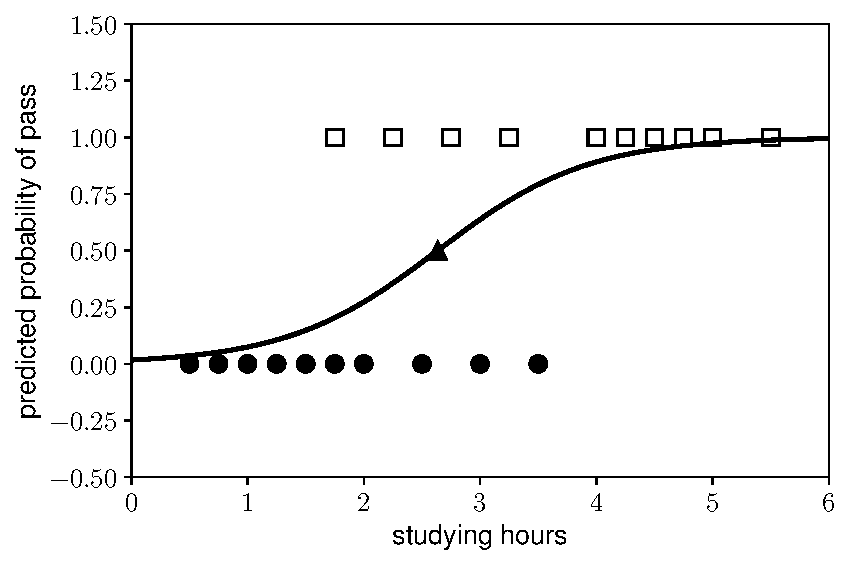
\includegraphics[width=0.99\linewidth]{ebookML_src/src/logistic_regression/log_reg_res.pdf}
\caption{}
\label{fig:10_resa}
\end{subfigure}
\begin{subfigure}{0.49\textwidth}
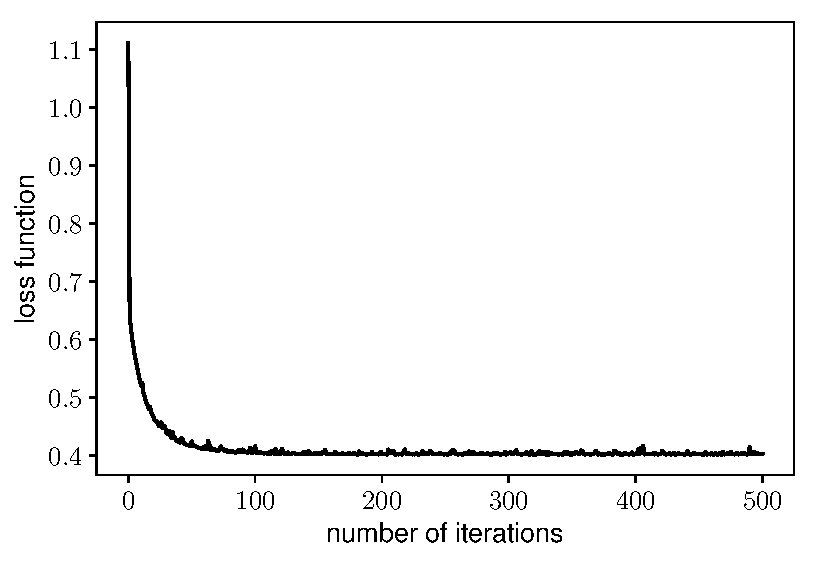
\includegraphics[width=0.99\linewidth]{ebookML_src/src/logistic_regression/log_reg_loss.pdf}
\caption{}
\label{fig:10_resb}
\end{subfigure}
\caption{
Nghiệm của hồi quy logistic cho bài toán dự đoán kết quả thi dựa trên
thời gian học. (a) Đường nét liền thể hiện xác suất thi đỗ dựa trên thời gian
học. Điểm tam giác thể hiện ngưỡng ra quyết định đỗ/trượt. Điểm này có
thể thay đổi tuỳ vào bài toán. (b) Giá trị của hàm mất mát qua các vòng lặp.
Hàm mất mát giảm nhanh và hội tụ sớm. }
\label{fig:10_res}
\end{figure}
%% *****************************************************************************

% <div class="imgcap">
% <img src ="\assets\LogisticRegression\lg_results.png" align = "center" width = "600">
% <div class = "thecap">Hình 4: Dữ liệu và hàm sigmoid tìm được.</div>
% </div>
% \begin{figure}[t]
%     % caption on side
%     \floatbox[{\capbeside\thisfloatsetup{capbesideposition={right,top},capbesidewidth=6cm}}]{figure}[\FBwidth]
%     {\caption{
%     Dữ liệu huấn luyện và hàm sigmoid tìm được.
%     }
%     \label{fig:10_4}}
%     { % figure here
%     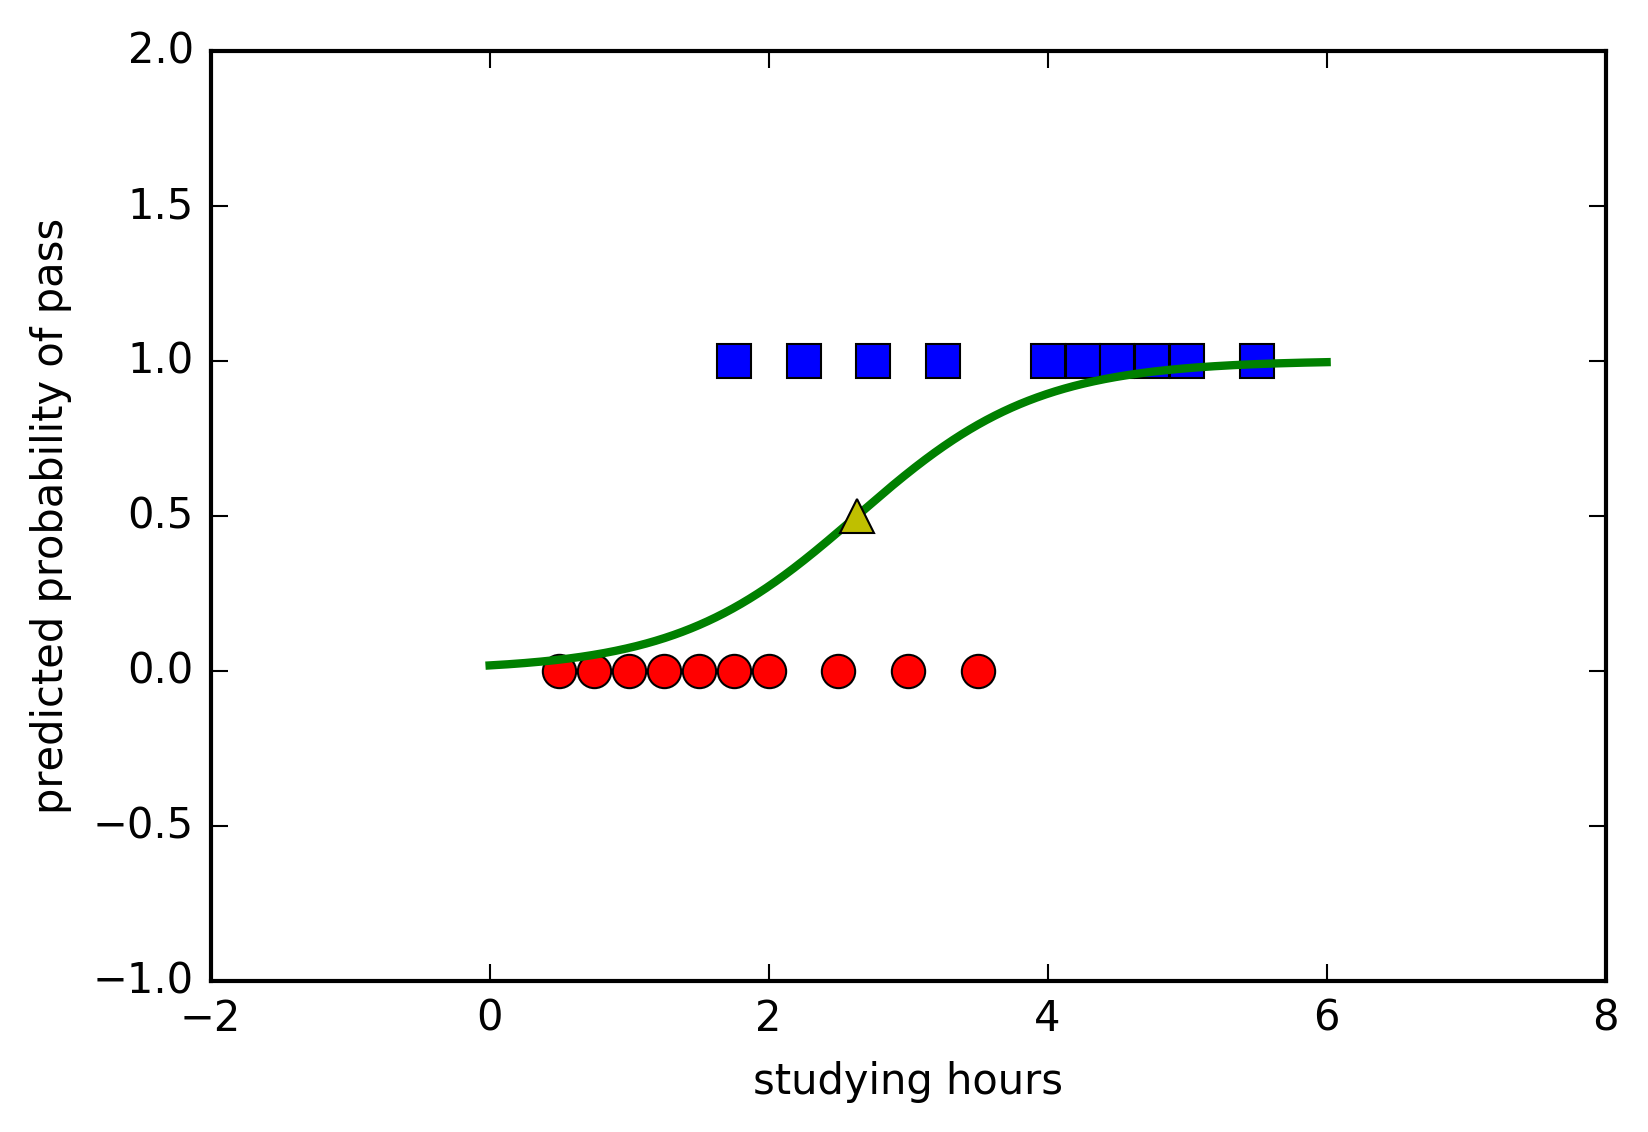
\includegraphics[width=.5\textwidth]{Chapters/05_NeuralNetworks/10_logisticregression/lg_results.png}
%     }
% \end{figure}





% Nếu như chỉ có hai output là \textit{fail} hoặc \textit{pass}, điểm trên đồ thị của hàm sigmoid tương ứng với xác suất 0.5 được chọn làm \textit{hard threshold} (ngưỡng cứng). Việc này có thể chứng minh khá dễ dàng (tôi sẽ bàn ở phần dưới).

% {\color{red} Bình luận }


\subsection{Ví dụ với dữ liệu hai chiều}
Giả sử có hai tập dữ liệu vuông và tròn phân bố trên mặt phẳng như trong Hình \ref{fig:10_logreg2da}. Với dữ liệu đầu vào nằm trong không gian hai chiều, hàm sigmoid có dạng thác nước như trong Hình~\ref{fig:10_logreg2db}.
% \begin{figure}[t]
%     % caption on side
%     \floatbox[{\capbeside\thisfloatsetup{capbesideposition={right,top},capbesidewidth=6cm}}]{figure}[\FBwidth]
%     {\caption{
%     Hàm sigmoid với dữ liệu có chiều là 2. (Nguồn: \href{http://galaxy.agh.edu.pl/~vlsi/AI/bias/bias_eng.html}{Biased and non biased neurons}.)
%     }
%     \label{fig:10_6}}
%     { % figure here
%     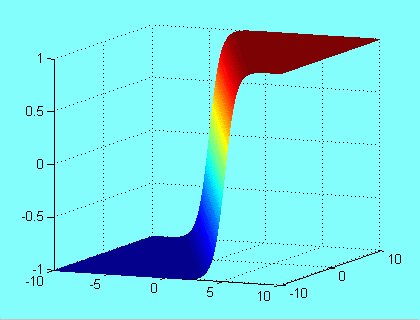
\includegraphics[width=.5\textwidth]{Chapters/05_NeuralNetworks/10_logisticregression/plaszczyzna.png}
%     }
% \end{figure}

%% *****************************************************************************
\begin{figure}[t]
\begin{subfigure}{0.49\textwidth}
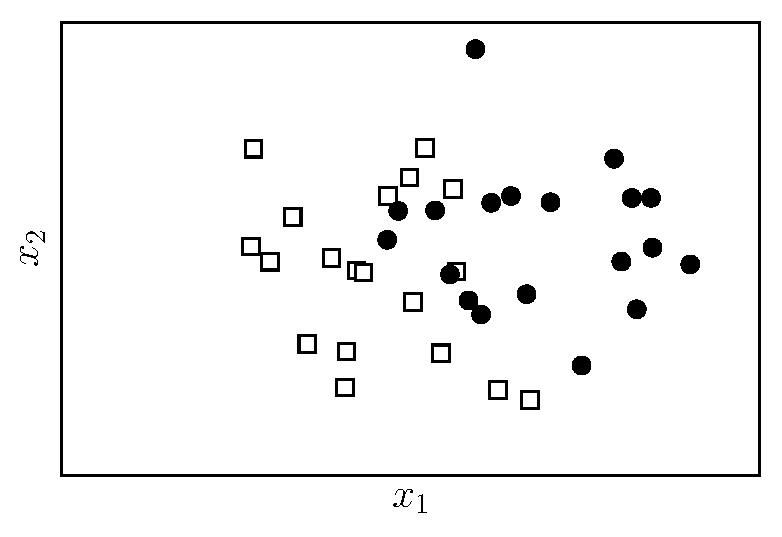
\includegraphics[width=0.99\linewidth]{ebookML_src/src/logistic_regression/logistic_2d.pdf}
\caption{Dữ liệu cho bài toán phân loại trong không gian hai chiều.}
\label{fig:10_logreg2da}
\end{subfigure}
\begin{subfigure}{0.45\textwidth}
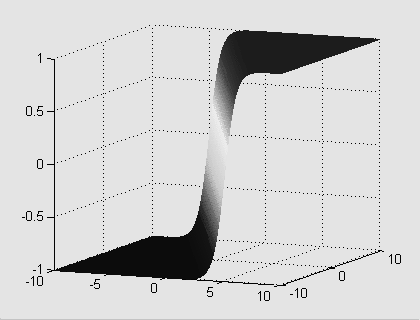
\includegraphics[width=0.99\linewidth]{Chapters/05_NeuralNetworks/10_logisticregression/plaszczyzna_gray.png}
\caption{Đồ thị hàm sigmoid trong không gian hai chiều (xem ảnh màu trong Hình~\ref{fig:10_logreg2db_c}).}
\label{fig:10_logreg2db}
\end{subfigure}
\caption{
Ví dụ về dữ liệu và hàm sigmoid trong không gian hai chiều.
}
\label{fig:10_logreg2d}
\end{figure}
%% *****************************************************************************



Kết quả dự đoán xác suất đầu ra khi áp dụng mô hình hồi quy logistic được minh họa như Hình
\ref{fig:10_7} với độ sáng của nền thể hiện xác suất điểm đó có nhãn tròn. Màu đen
đậm thể hiện giá trị gần bằng không, màu trắng thể hiện giá trị rất gần bằng một.

\begin{figure}[t]
% caption on side
\floatbox[{\capbeside\thisfloatsetup{capbesideposition={right,top},capbesidewidth=6cm}}]{figure}[\FBwidth]
{\caption{
Ví dụ về hồi quy logistic với dữ liệu hai chiều. Vùng màu càng đen thể hiện xác suất thuộc nhãn hình vuông càng cao. Vùng màu càng trắng thể hiện xác suất thuộc nhãn hình tròn càng cao. Vùng biên giữa hai nhãn (khu vực màu xám) thể hiện các điểm thuộc vào mỗi nhãn với xác suất thấp hơn.    }
\label{fig:10_7}}
{ % figure here
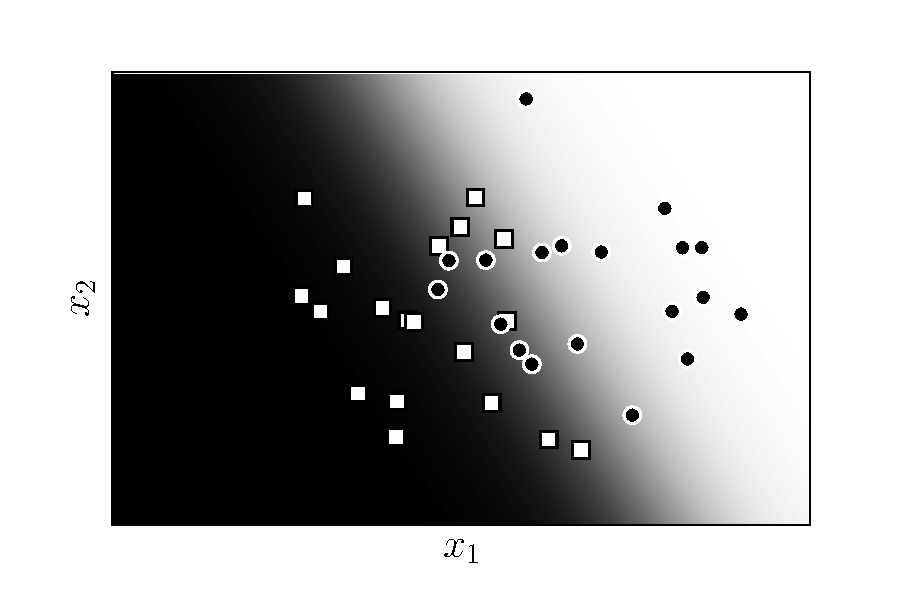
\includegraphics[width=.5\textwidth]{ebookML_src/src/logistic_regression/logistic_2d_2.pdf}
}
\end{figure}

Nếu phải lựa chọn một ranh giới thay vì xác suất, ta thấy các đường thẳng nằm
trong khu vực màu xám là các lựa chọn hợp lý. Ta sẽ chứng minh ở phần sau rằng
tập hợp các điểm có cùng xác suất đầu ra tạo thành một siêu phẳng.

Mã nguồn cho chương này có thể được tìm thấy tại
\url{https://goo.gl/9e7sPF}.

Cách sử dụng hồi quy logistic trong thư viện scikit-learn có thể được tìm thấy tại \url{https://goo.gl/BJLJNx}.


\section{Tính chất của hồi quy logistic}
\begin{enumerate}
\item \textit{Hồi quy logistic thực ra là một thuật toán phân loại.}

Mặc dù trong tên có từ \textit{hồi quy}, hồi quy logistic được sử dụng nhiều
trong các bài toán phân loại. Sau khi tìm được mô hình, việc xác định
nhãn $y$ cho một điểm dữ liệu $\bx$ được xác định bằng việc so sánh
hai giá trị:
\begin{equation}
P(y = 1| \bx; \bw); ~~ P(y = 0| \bx; \bw)
\end{equation}
Nếu giá trị thứ nhất lớn hơn, ta kết luận điểm dữ liệu có nhãn một và
ngược lại. Vì tổng hai giá trị này luôn bằng một nên ta chỉ cần xác định
$P(y = 1| \bx; \bw)$ có lớn hơn 0.5 hay không.



% \newpage
\item \textit{Đường ranh giới tạo bởi hồi quy logistic là một siêu phẳng.}

Thật vậy, giả sử những điểm có xác suất đầu ra lớn hơn 0.5 được gán nhãn một. Tập hợp các điểm này là nghiệm của bất phương trình:
\begin{eqnarray*}
P(y = 1| \bx; \bw) > 0.5
\Leftrightarrow \frac{1}{1 + e^{-\bx^T\bw}} > 0.5
\Leftrightarrow e^{-\bx^T\bw} < 1
\Leftrightarrow \bx^T\bw > 0
\end{eqnarray*}
Nói cách khác, tập hợp các điểm được gán nhãn một tạo thành một nửa không gian $\bx^T\bw > 0$, tập hợp các điểm được gán nhãn không tạo thành nửa không gian còn lại. Ranh giới giữa hai nhãn là siêu phẳng $\bx^T\bw = 0$.

Vì vậy, hồi quy logistic được coi như một bộ phân loại tuyến tính.

\item \textit{Hồi quy logistic không yêu cầu giả thiết tách biệt tuyến tính.}

Một điểm cộng của hồi quy logistic so với PLA là nó không cần giả thiết dữ liệu hai tập hợp là tách biệt tuyến tính. Tuy nhiên, ranh giới tìm được vẫn có dạng tuyến tính. Vì vậy, mô hình này chỉ phù hợp với loại dữ liệu mà hai tập \textit{gần} tách biệt tuyến tính.

\item \textit{Ngưỡng ra quyết định có thể thay đổi.}

Hàm dự đoán đầu ra của các điểm dữ liệu mới có thể được viết như sau:
\begin{lstlisting}[language=Python]
def predict(w, X, threshold = 0.5):
"""
predict output for each row of X
X: a numpy array of shape (N, d), threshold: 0 < threshold < 1
return a 1d numpy array, each element is 0 or 1
"""
res = np.zeros(X.shape[0])
res[np.where(prob(w, X) > threshold)[0]] = 1
return res
\end{lstlisting}
Trong các ví dụ đã nêu, ngưỡng ra quyết định đều được lấy tại 0.5. Trong
nhiều trường hợp, ngưỡng này có thể được thay đổi. Ví dụ, việc xác định các
giao dịch là lừa đảo của một công ty tín dụng là rất quan trọng. Việc phân
loại nhầm một giao dịch lừa đảo thành một giao dịch thông thường gây ra hậu
quả nghiêm trọng hơn chiều ngược lại. Trong bài toán đó, ngưỡng phân loại có
thể giảm xuống còn 0.3. Nghĩa là các giao dịch được dự đoán là lừa đảo với
xác suất lớn hơn 0.3 sẽ được gán nhãn lừa đảo và cần được xử lý bằng các biện pháp khác.



\item Khi biểu diễn dưới dạng các mạng neuron, hồi quy tuyến tính, PLA và
hồi quy logistic có thể được biểu diễn như trong Hình~\ref{fig:10_8}. Sự
khác nhau chỉ nằm ở lựa chọn hàm kích hoạt.
\begin{figure}[t]
\centering
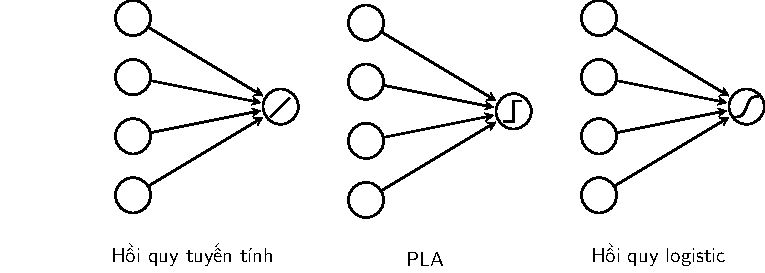
\includegraphics[width = .9\textwidth]{Chapters/05_NeuralNetworks/10_logisticregression/latex/3models.pdf}
% \includegraphics[width = \textwidth]{}
\caption[]{Biểu diễn hồi quy tuyến tính, PLA, và hồi quy logistic
dưới dạng neural network.}
\label{fig:10_8}
\end{figure}

\end{enumerate}










\section{Bài toán phân biệt hai chữ số viết tay }
Xét bài toán phân biệt hai chữ số không và một trong bộ cơ sở dữ liệu MNIST.
Trong mục này, class \pythoninline{LogisticRegression} trong thư viện
scikit-learn sẽ được sử dụng. Trước tiên, ta cần khai báo các thư viện và tải về
bộ cơ sở dữ liệu MNIST:


\begin{lstlisting}[language=Python]
import numpy as np
from sklearn.datasets import fetch_mldata
from sklearn.model_selection import train_test_split
from sklearn.linear_model import LogisticRegression
from sklearn.metrics import accuracy_score
mnist = fetch_mldata('MNIST original', data_home='../../data/')
N, d = mnist.data.shape
print('Total {:d} samples, each has {:d} pixels.'.format(N, d))
\end{lstlisting}
\kq
\begin{lstlisting}[language=Python]
Total 70000 samples, each has 784 pixels.
\end{lstlisting}

Có tổng cộng 70000 điểm dữ liệu trong tập dữ liệu MNIST, mỗi điểm là một mảng
784 phần tử tương ứng với 784 pixel. Mỗi chữ số từ không đến chín chiếm khoảng
mười phần trăm. Chúng ta sẽ lấy ra tất cả các điểm ứng với chữ số không và một,
sau đó chọn ngẫu nhiên 2000 điểm làm tập kiểm tra, phần còn lại đóng vai trò
tập huấn luyện.
\begin{lstlisting}[language=Python]
X_all = mnist.data
y_all = mnist.target
X0 = X_all[np.where(y_all == 0)[0]] # all digit 0
X1 = X_all[np.where(y_all == 1)[0]] # all digit 1
y0 = np.zeros(X0.shape[0]) # class 0 label
y1 = np.ones(X1.shape[0])  # class 1 label
X = np.concatenate((X0, X1), axis = 0) # all digits 0 and 1
y = np.concatenate((y0, y1)) # all labels
# split train and test
X_train, X_test, y_train, y_test = train_test_split(X, y, test_size=2000)
\end{lstlisting}

Tiếp theo, ta xây dựng mô hình hồi quy logistic trên tập huấn luyện và dự
đoán nhãn của các điểm trong tập kiểm tra. Kết quả này được so sánh với nhãn
thực sự của mỗi điểm dữ liệu để tính độ chính xác của bộ phân loại:
\begin{lstlisting}[language=Python]
model = LogisticRegression(C = 1e5) # C is inverse of lam
model.fit(X_train, y_train)
y_pred = model.predict(X_test)
print("Accuracy %.2f %%" % (100*accuracy_score(y_test, y_pred.tolist())))
\end{lstlisting}
\kq
\begin{lstlisting}[language=Python]
Accuracy 99.90 %
\end{lstlisting}
Như vậy, gần 100\% các ảnh được phân loại chính xác. Điều này dễ hiểu vì hai
chữ số không và một khác nhau rất nhiều.

Tiếp theo, ta cùng đi tìm những ảnh bị phân loại sai và hiển thị chúng:
\begin{lstlisting}[language=Python]
mis = np.where((y_pred - y_test) !=0)[0]
Xmis = X_test[mis, :]
from display_network import *
filename = 'mnist_mis.pdf'
with PdfPages(filename) as pdf:
plt.axis('off')
A = display_network(Xmis.T, 1, Xmis.shape[0])
f2 = plt.imshow(A, interpolation='nearest' )
plt.gray()
pdf.savefig(bbox_inches='tight')
plt.show()
\end{lstlisting}

%% *****************************************************************************
\begin{figure}[t]
% caption on side

\floatbox[{\capbeside\thisfloatsetup{capbesideposition={right,top},capbesidewidth=7cm}}]{figure}[\FBwidth]
{\caption{
Các chữ số bị phân loại lỗi trong bài toán phân loại nhị phân với hai chữ số không và một.
}
\label{fig:10_mnist_miss}}
{ % figure here

\includegraphics[width=.4\textwidth]{ebookML_src/src/logistic_regression/mnist_mis.pdf}
}
\end{figure}
%% *****************************************************************************
Chỉ có hai chữ số bị phân loại lỗi được cho trên Hình~\ref{fig:10_mnist_miss}.
Trong đó, chữ số không bị phân loại lỗi là dễ hiểu vì nó trông rất giống chữ số một.
% <div class="imgcap">
% <img src ="\assets\LogReg2\0.png" align = "center" width = "100">
% <div class = "thecap">Hình 3: Chữ số bị phân loại sai trong bài toán phân loại ảnh chữ số 0 và 1</div>
% </div>
% \begin{figure}[t]
%     % caption on side
%     \floatbox[{\capbeside\thisfloatsetup{capbesideposition={right,top},capbesidewidth=12cm}}]{figure}[\FBwidth]
%     {\caption{
%     Chữ số bị phân loại sai trong bài toán phân loại ảnh chữ số 0 và 1.
%     }
%     \label{fig:10_3}}
%     { % figure here
%     
\includegraphics[width=.15\textwidth]{Chapters/05_NeuralNetworks/12_binaryclassifiers/0.png}
%     }
% \end{figure}

% Như vậy là chỉ có một ảnh bị phân loại sai. Ảnh này là chữ số 0 nhưng bị misclassified thành chữ số 1, có thể vì nét đậm nhất của nó rất giống với chữ số 1.

% Source code cho ví dụ này có thể được tìm thấy \href{http://machinelearningcoban.com/assets/LogReg2/LogReg2.ipynb}{ở đây}.

Bạn đọc có thể xem thêm ví dụ về bài toán xác định giới tính dựa trên ảnh
khuôn mặt tại \url{https://goo.gl/9V8wdD}.

\section{Bài toán phân loại đa lớp}
\label{sec:biclassifier}
\index{phân loại đa lớp -- multi-class classification}
\index{multi-class classification -- phân loại đa lớp}
% Có lẽ nhiều bạn đang đặt câu hỏi: Các ví dụ trên đây đều làm với bài toán có hai classes. Vậy nếu có nhiều hơn hai classes, ví dụ như 10 classes của MNIST, thì làm thế nào?
Hồi quy logistic được áp dụng cho các bài toán phân loại nhị phân. Các bài
toán phân loại thực tế có thể có nhiều hơn hai nhãn dữ liệu, được gọi
là bài toán \textit{phân loại đa lớp} (\textit{multi-class classification}). Hồi quy logistic cũng có thể được áp dụng vào các bài toán này bằng một vài kỹ thuật.

% Có nhiều thuật toán khác được xây dựng riêng cho các bài toán với nhiều classes (multi-class classification problems), tôi sẽ giới thiệu sau. Còn bây giờ, chúng ta vẫn có thể sử dụng các \textit{binary classifiers} để thực hiện công việc này, với một chút thay đổi.

Có {ít nhất} bốn cách áp dụng các bộ phân loại nhị phân vào bài toán phân
loại đa lớp.% Từ đây,
% \textit{binary classifier} và \textit{multi-class classification} sẽ được dùng
% xen kẽ với \textit{bộ phân loại nhị phân} và \textit{phân loại đa lớp}.

\subsection{one-vs-one}
\index{one-vs-one}

Ta có thể xây dựng nhiều bộ phân loại nhị phân cho từng cặp hai nhãn dữ liệu. Bộ
thứ nhất phân biệt nhãn thứ nhất và nhãn thứ hai, bộ thứ hai phân biệt nhãn thứ
nhất và nhãn thứ ba,... Có tổng cộng $P = \frac{C(C-1)}{2}$ bộ phân loại nhị phân
cần xây dựng với $C$ là số lượng nhãn. Cách thực hiện này được gọi là
\textit{one-vs-one}.

Với một điểm dữ liệu kiểm tra, ta dùng tất cả $P$ bộ phân loại để dự đoán nhãn của nó. Kết quả cuối cùng có thể được xác định bằng cách
xem điểm dữ liệu đó được gán nhãn nào nhiều nhất. Ngoài ra, nếu mỗi bộ phân loại có thể đưa ra xác suất giống hồi quy logistic, ta có thể tính {tổng các xác suất} mà điểm dữ liệu đó rơi vào mỗi nhãn. Chú ý rằng tổng các xác suất là $P$ thay vì một bởi có $P$ bộ phân loại khác nhau.


Cách làm này không lợi về tính toán vì số bộ phân loại phải huấn luyện tăng
nhanh khi số nhãn tăng lên. Hơn nữa, điều không hợp lý xảy ra nếu một chữ số có nhãn bằng một được đưa vào bộ phân loại giữa hai nhãn chữ số năm và sáu.

\subsection{Phân loại phân tầng}
\index{phân loại phân tầng -- hierarchical classification}
\index{hierarchical classification -- phân loại phân tầng}
One-vs-one yêu cầu xây dựng $\frac{C(C-1)}{2}$ bộ phân loại khác nhau. Để giảm
số bộ phân loại cần xây dựng, ta có thể dùng phương pháp \textit{phân tầng}. Ý
tưởng của phương pháp này có thể được thấy qua ví dụ sau.

Xét bài toán phân loại bốn chữ số \{4, 5, 6, 7\} trong
MNIST. Vì chữ số {4} và {7} khá giống nhau, chữ số
{5} và {6} khá giống nhau nên trước tiên ta xây dựng
bộ phân loại giữa \{4, 7\} và \{5, 6\}. Sau đó xây dựng thêm hai bộ phân loại
để xác định từng chữ số trong mỗi nhóm. Tổng cộng, ta cần ba bộ phân loại nhị phân so với sáu bộ như khi sử dụng one-vs-one.

Có nhiều cách chia nhỏ tập dữ liệu ban đầu ra các cặp tập con. Cách phân tầng có ưu điểm là giảm số bộ phân loại nhị phân cần xây dựng. Tuy nhiên, cách làm này có một hạn chế lớn: nếu chỉ một bộ phân loại cho kết quả sai thì kết quả cuối cùng chắc chắn sẽ sai. Ví dụ, nếu một ảnh chứa chữ
số {5} bị phân loại lỗi bởi bộ phân loại đầu tiên thì cuối cùng nó sẽ bị nhận nhầm thành 4 hoặc 7.


\subsection{Mã hoá nhị phân}
Có một cách tiếp tục giảm số bộ phân loại là \textit{mã hoá nhị phân}. Trong phương pháp này, mỗi nhãn được mã hoá bởi một số nhị phân. Ví dụ, nếu có bốn nhãn thì chúng được mã hoá bởi 00, 01, 10, và 11. Số bộ phân loại nhị phân cần xây dựng chỉ là $m =
\left\lceil\log_2(C)\right\rceil$ trong đó $C$ là số nhãn, $\left\lceil a
\right\rceil$ là {số nguyên nhỏ nhất không nhỏ hơn} $a$. Bộ phân loại đầu tiên giúp xác định bit đầu tiên của nhãn, bộ thứ hai xác định bit tiếp theo,....
Cách làm này sử dụng một số lượng nhỏ nhất các bộ phân loại nhị phân. Tuy
nhiên, một điểm dữ liệu chỉ được phân loại đúng khi mọi bộ phân loại nhị phân dự đoán đúng bit tương ứng. Hơn nữa, nếu số nhãn không phải là lũy thừa của hai,
mã nhị phân nhận được có thể không tương ứng với nhãn nào.


\subsection{one-vs-rest}
\index{one-vs-rest}
Kỹ thuật được sử dụng nhiều nhất là \textit{one-vs-rest}\footnote{Một số tài
liệu gọi là \textit{ove-vs-all}, \textit{one-against-rest}, hoặc
\textit{one-against-all}.}. Cụ thể, $C$ bộ phân loại nhị phân được xây dựng
tương ứng với các nhãn. Bộ thứ nhất xác định một điểm có nhãn thứ nhất hay
không, hoặc xác suất để một điểm có nhãn đó. Tương tự, bộ thứ hai xác định điểm
đó có nhãn thứ hai hay không hoặc xác xuất có nhãn thứ hai là bao nhiêu. Nhãn
cuối cùng được xác định theo nhãn mà điểm đó rơi vào với xác suất cao nhất.


% \index{one-hot coding}
% Phương pháp này còn được gọi là \textbf{one-hot coding} vì với cách mã hóa
% trên, giả sử có 4 classes, class 1, 2, 3, 4 sẽ lần lượt được mã hóa dưới dạng nhị phân bởi \pythoninline{1000, 0100, 0010} hoặc \pythoninline{0001}. One-hot vì chỉ có \textit{one} bit là \textit{hot} (bằng \pythoninline{1}).

Hồi quy logistic trong thư viện scikit-learn có thể được áp dụng trực tiếp
vào các bài toán phân loại đa lớp với kỹ thuật {one-vs-rest}. Với MNIST, ta có thể dùng hồi quy logistic kết hợp với one-vs-rest (mặc định) như sau:
\begin{lstlisting}[language=Python]
X_train, X_test, y_train, y_test = \
train_test_split(X_all, y_all, test_size=10000)
model = LogisticRegression(C = 1e5) # C is inverse of lam
model.fit(X_train, y_train)
y_pred = model.predict(X_test)
print("Accuracy %.2f %%" % (100*accuracy_score(y_test, y_pred.tolist())))
\end{lstlisting}

Kết quả thu được tương đối thấp, khoảng 91.7\%. Phương pháp KNN đơn giản hơn đã
có độ chính xác khoảng 96\%. Điều này chứng tỏ one-vs-rest không làm việc tốt
trong trường hợp này.

% Một chú ý nhỏ: kỹ thuật mặc định cho các bài toán multi-class của hàm này được xác định bởi biến \pythoninline{multi_class}. Có hai lựa chọn cho biến này, trong đó lựa chọn mặc định là \pythoninline{ovr} tức \textbf{one-vs-rest}, lựa chọn còn lại sẽ được tôi đề cập trong một bài gần đây. Lựa chọn thứ hai không phải cho binary classifiers nên tôi không đề cập trong bài này, có thể sau một vài bài nữa (Xem thêm \href{http://scikit-learn.org/stable/modules/generated/sklearn.linear_model.LogisticRegression.html}{\pythoninline{sklearn.linear_model.LogisticRegression}})



\section{Thảo luận }

\subsection{Kết hợp các phương pháp trên}
% Khái niệm tách biệt tuyến tính có thể được mở rộng để áp dụng cho nhiều lớp dữ
% liệu. Nếu hai lớp bất kỳ trong nhiều lớp dữ liệu là tách biệt tuyến tính, ta nói
% các lớp đó là tách biệt tuyến tính.

% Nhắc lại rằng các linear binary classifiers tôi đã trình bày yêu cầu dữ liệu là \textit{tách biệt tuyến tính} hoặc \textit{nearly tách biệt tuyến tính}. Ta cũng có thể mở rộng định nghĩa này cho các bài toán multi-class. Nếu hai class bất kỳ là \textit{tách biệt tuyến tính} thì ta coi dữ liệu đó là \textit{tách biệt tuyến tính}.

Trong nhiều trường hợp, ta cần kết hợp nhiều kỹ thuật trong số bốn kỹ thuật đã
đề cập. Xét ba ví dụ trong Hình \ref{fig:10_4}.

\begin{figure}[t]
\centering
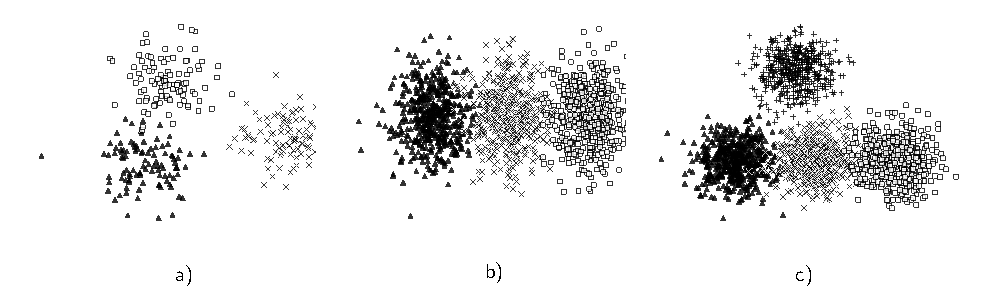
\includegraphics[width = \textwidth]{Chapters/05_NeuralNetworks/12_binaryclassifiers/latex/dist.pdf}
\caption[]{Ví dụ về phân phối của các tập dữ liệu trong bài toán
phân loại đa lớp.}
\label{fig:10_4}
\end{figure}
\begin{itemize}
\item Hình~\ref{fig:10_4}a: Cả bốn phương pháp trên đây đều có thể áp dụng được.

\item Hình~\ref{fig:10_4}b: One-vs-rest không phù hợp vì tập dữ liệu ở giữa và
hợp của hai tập còn lại là không (gần) {tách biệt tuyến tính}. Lúc này,
one-vs-one hoặc phân tầng phù hợp hơn.

\item Hình~\ref{fig:10_4}c: Tương tự như trên, có ba tập dữ liệu thẳng hàng
nên one-vs-rest sẽ không phù hợp. Trong khi đó, one-vs-one vẫn hiệu quả vì
từng cặp nhãn dữ liệu là (gần) {tách biệt tuyến tính}. Tương tự, phân tầng cũng
làm việc nếu ta phân chia các nhãn một cách hợp lý. Ta cũng có thể kết hợp
nhiều phương pháp. Ví dụ, dùng one-vs-rest để tách nhãn ở hàng trên ra khỏi ba nhãn
thẳng hàng ở dưới. Ba nhãn còn lại có thể tiếp tục được phân loại bằng các phương pháp khác. Tuy nhiên, khó khăn vẫn nằm ở việc phân nhóm như thế nào.
\end{itemize}

Với bài toán phân loại đa lớp, nhìn chung các kỹ thuật sử dụng các bộ phân loại
nhị phân ít mang lại hiệu quả. Mời bạn đọc thêm
Chương~\ref{cha:softmax} và Chương~\ref{cha:multisvm} để tìm hiểu về các bộ phân
loại đa lớp phổ biến nhất hiện nay.

% Bạn đọc có thể xem thêm ví dụ áp dụng Logistic Regression cho cơ sở dữ
% liệu \href{http://machinelearningcoban.com/2017/01/08/knn/#bo-co-so-du-lieu-iris-iris-flower-dataset}{Iris} trong \href{http://scikit-learn.org/stable/auto_examples/linear_model/plot_iris_logistic.html}{link này}



% <div class="imgcap">
% <img src ="http://scikit-learn.org/stable/_images/sphx_glr_plot_iris_logistic_001.png" align = "center" width = "500">
% <div class = "thecap">Hình 5: Logistic Regression với Iris database. (Nguồn: <a href="http://scikit-learn.org/stable/auto_examples/linear_model/plot_iris_logistic.html">Logistic Regression 3-class Classifier</a>)</div>
% </div>
%% *****************************************************************************
\begin{figure}[t]
% caption on side
\floatbox[{\capbeside\thisfloatsetup{capbesideposition={right,top},capbesidewidth=3cm}}]{figure}[\FBwidth]
{\caption{
Mô hình neural network cho các kỹ thuật sử dụng các bộ phân loại nhị phân
cho bài toán phân loại đa lớp.
}
\label{fig:12_6}}
{ % figure here
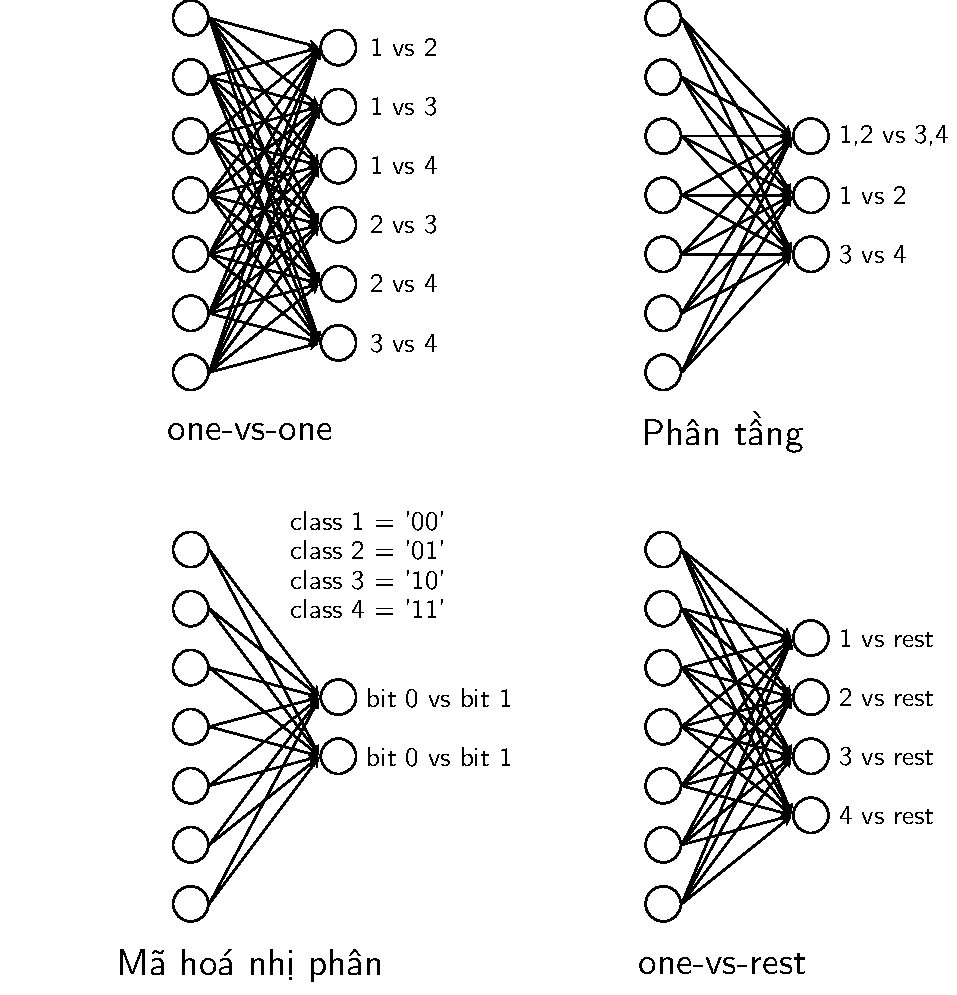
\includegraphics[width=.63\textwidth]{Chapters/05_NeuralNetworks/12_binaryclassifiers/latex/binaryclassifiers.pdf}
}
\end{figure}
%% *****************************************************************************
\subsection{Biểu diễn dưới dạng mạng neuron}
Lấy ví dụ bài toán có bốn nhãn dữ liệu \{1, 2, 3, 4\}; ta có thể biểu diễn các kỹ
thuật đã được đề cập dưới dạng mạng neuron như trong Hình~\ref{fig:12_6}. Mỗi nút ở tầng đầu ra thể hiện đầu ra của một bộ phân loại nhị phân.

\index{ma trận trọng số -- weight matrix}
\index{weight matrix -- ma trận trọng số}
Các mạng neuron này đều có nhiều nút ở tầng đầu ra, vector trọng số
$\bw$ đã trở thành \textit{ma trận trọng số} $\mathbf{W}$. Mỗi
cột của $\bW$ tương ứng với vector trọng số của một nút đầu ra. Các bộ phân loại nhị phân này có thể được xây dựng đồng thời. Nếu chúng là các bộ hồi quy logistic, công thức cập nhật theo SGD:
\begin{equation}
\bw \assign \bw - \eta(a_i - y_i)\bx_i
\end{equation}
có thể được tổng quát thành
\begin{equation}
\label{eqn:gen_sgd_log}
\mathbf{W} \assign \mathbf{W} - \eta\bx_i(\mathbf{a}_i - \mathbf{y}_i)^T.
\end{equation}
Với $\mathbf{W}, \mathbf{y}_i, \mathbf{a}_i$ lần lượt là ma trận trọng số,
vector đầu ra thực sự và vector đầu ra dự đoán ứng với dữ liệu $\bx_i$. Chú ý
rằng vector $\mathbf{y}_i$ là một vector nhị phân, vector $\mathbf{a}_i$ gồm các
phần tử nằm trong khoảng $(0, 1)$.


\textit{Chú ý}: Số hạng thứ hai trong~\eqref{eqn:gen_sgd_log} không thể là $(\ba_i - \by_i)\bx_i^T$ vì ma trận này khác chiều với $\bW$. Số hạng này cần là tích của hai vector: vector thứ nhất cần có cùng số hàng với $\bW$, tức chiều của dữ liệu $\bx_i$; vector thứ hai cần phù hợp với số cột của $\bW$, tức số nút ở tầng đầu ra.



% \subsection{Hạn chế của one-vs-rest}
% Xem xét lại phương pháp one-vs-rest theo góc nhìn xác suất, một điểm dữ liệu có thể được dự đoán thuộc vào class $1, 2, \dots, C$ với xác suất lần lượt là $p_1, p_2, \dots, p_C$. Tuy nhiên, tổng các xác suất này có thể không bằng 1! Có một phương pháp có thể làm cho nó \textit{hợp lý hơn}, tức \textit{ép} tổng các xác suất này bằng 1. Khi đó, với 1 điểm dữ liệu ta có thể nói xác suất nó rơi vào mỗi class là bao nhiêu. Phương pháp hấp dẫn này sẽ được đề cập trong bài \href{http://machinelearningcoban.com/2017/02/16/softmax/}{Softmax Regression}. Mời bạn đón đọc.



% \subsection{Đọc thêm}
% \begin{enumerate}
%     \item D. Cox, \textit{The regression analysis of binary sequences.}
%     Journal of the Royal Statistical Society. Series B (Methodological) (1958): 215-242.

% [2] Cramer, Jan Salomon. "The origins of hồi quy logistic." (2002).

% [3] Abu-Mostafa, Yaser S., Malik Magdon-Ismail, and Hsuan-Tien Lin. Learning from data. Vol. 4. New York, NY, USA:: AMLBook, 2012. (\href{http://work.caltech.edu/telecourse.html}{link to course})

% [4] Bishop, Christopher M. "Pattern recognition and Machine Learning.", Springer  (2006). %(\href{http://users.isr.ist.utl.pt/~wurmd/Livros/school/Bishop%20-%20Pattern%20Recognition%20And%20Machine%20Learning%20-%20Springer%20%202006.pdf}{book})

% [5] Duda, Richard O., Peter E. Hart, and David G. Stork. Pattern classification. John Wiley \& Sons, 2012.

% [6] Andrer Ng. CS229 Lecture notes. \href{https://datajobs.com/data-science-repo/Generalized-Linear-Models-[Andrew-Ng].pdf}{Part II: Classification and hồi quy logistic}

% [7] Jerome H. Friedman, Robert Tibshirani, and Trevor Hastie. \href{https://statweb.stanford.edu/~tibs/}{The Elements of Statistical Learning}.
% \end{enumerate}

% [1] \href{https://en.wikipedia.org/wiki/Multiclass_classification}{Multiclass classification - wiki}

% [2] \href{http://scikit-learn.org/stable/auto_examples/linear_model/plot_iris_logistic.html}{Logistic Regression 3-class Classifier}
